%% FullCourse_10Lecs -- Lecture 6, Topic 6.1: Aiyagari--Bewley--Huggett + Stationary Eq Computation
%% Source: ./archive_pre_split/Lec06_HA_Models.tex (sections 1-2)
%% Pass B addition: Bilibili footnote on classical HA computation methods (Step 3 algorithm).

%% Shared preamble for the FullCourse_10Lecs topic decks.
%%
%% Each topic .tex \input's this file, then defines its own \title, \date
%% override (if any), \graphicspath, and \begin{document}.
%%
%% Reconstructed verbatim from the inlined copy preserved in
%% Lec10_Case_Studies/Lec10_T8_Case6_DeepRamsey.tex (lines 23-190), which is
%% explicitly annotated there as "from ../shared_preamble.tex, copied verbatim".
%% Base preamble matches MiniCourse_8hr/Slides/shared_preamble.tex; this version
%% additionally provides \sectiondivider, the conceptbox/cautionbox/examplebox/
%% takeawaybox tcolorboxes, and \compacttables used across the split decks.

\documentclass[10pt,english,aspectratio=169]{beamer}

\usepackage{ae,aecompl}
\usepackage[T1]{fontenc}
\usepackage{textcomp}
\usepackage[utf8]{inputenc}
\usepackage{babel}
\usepackage{datetime2}

\setcounter{secnumdepth}{3}
\setcounter{tocdepth}{3}

\usepackage{amsmath, amssymb, amsthm, graphicx}
\usepackage{booktabs, multirow}
\usepackage{tikz}
\usepackage{pgfplots}
\pgfplotsset{compat=1.16}
\usepackage[most]{tcolorbox}
\tcbuselibrary{skins, breakable, theorems}
\usepackage{listings}
\usepackage{xcolor}

\lstset{
  basicstyle=\ttfamily\small,
  keywordstyle=\color{blue!80!black}\bfseries,
  commentstyle=\color{green!50!black}\itshape,
  stringstyle=\color{orange!80!black},
  backgroundcolor=\color{gray!8},
  frame=single,
  rulecolor=\color{gray!40},
  breaklines=true,
  showstringspaces=false,
  numbers=none,
}

\lstdefinestyle{pythonstyle}{
    language=Python,
    basicstyle=\ttfamily\footnotesize,
    keywordstyle=\color{blue!80!black}\bfseries,
    commentstyle=\color{green!50!black}\itshape,
    stringstyle=\color{orange!80!black},
    frame=single,
    breaklines=true,
    showstringspaces=false,
    numbers=left,
    numbersep=5pt,
    numberstyle=\tiny\color{gray},
    backgroundcolor=\color{gray!8},
    rulecolor=\color{gray!40}
}

\ifx\hypersetup\undefined
  \AtBeginDocument{%
    \hypersetup{bookmarks=false,breaklinks=true,pdfborder={0 0 0},colorlinks=true,
      linkcolor=DarkText,urlcolor=RedTitle}%
  }
\else
  \hypersetup{bookmarks=false,breaklinks=true,pdfborder={0 0 0},colorlinks=true,
    linkcolor=DarkText,urlcolor=RedTitle}%
\fi

\makeatletter
\newcommand\makebeamertitle{%
  \begin{frame}[plain]
    \vspace*{1.0cm}
    \centering
    {\usebeamerfont{title}\usebeamercolor[fg]{title}\inserttitle\par}
    \vspace{1.0cm}
    {\usebeamerfont{author}\usebeamercolor[fg]{author}\insertauthor\par}
    \vspace{0.2cm}
    {\usebeamerfont{date}\usebeamercolor[fg]{date}\insertdate\par}
  \end{frame}}%
\AtBeginDocument{%
  \let\origtableofcontents=\tableofcontents
  \def\tableofcontents{\@ifnextchar[{\origtableofcontents}{\gobbletableofcontents}}
  \def\gobbletableofcontents#1{\origtableofcontents}%
}

\usetheme{metropolis}
\usefonttheme{professionalfonts}

\definecolor{LightGray}{RGB}{230,230,230}
\definecolor{RedTitle}{RGB}{0,0,200}
\definecolor{VeryLightGray}{RGB}{245,245,245}
\definecolor{DarkText}{RGB}{0,0,0}

\setbeamercolor{background canvas}{bg=white}
\setbeamercolor{title}{fg=RedTitle}
\setbeamercolor{author}{fg=DarkText}
\setbeamercolor{date}{fg=DarkText}
\setbeamercolor{frametitle}{bg=VeryLightGray,fg=DarkText}
\setbeamercolor{normal text}{fg=DarkText}
\setbeamerfont{title}{size=\large}

\setbeamersize{text margin left=5mm, text margin right=5mm}
\addtobeamertemplate{frametitle}{}{\vspace{-0.5em}}
\newcommand{\reducevspace}{\vspace{-0.5cm}}

% Shared section divider and box styles for split topic decks.
\newcommand{\sectiondivider}[2]{%
\begin{frame}[plain,noframenumbering]
\begin{center}
\vfill
{\Large\textbf{#1}\par}
\vspace{0.35cm}
{\normalsize #2\par}
\vfill
\end{center}
\end{frame}
}

\newtcolorbox{conceptbox}[1][]{
  colback=blue!3,
  colframe=RedTitle!55,
  boxrule=0.35mm,
  arc=1mm,
  left=2mm,
  right=2mm,
  top=1mm,
  bottom=1mm,
  #1
}
\newtcolorbox{cautionbox}[1][]{
  colback=red!3,
  colframe=red!50!black,
  boxrule=0.35mm,
  arc=1mm,
  left=2mm,
  right=2mm,
  top=1mm,
  bottom=1mm,
  #1
}
\newtcolorbox{examplebox}[1][]{
  colback=green!3,
  colframe=green!45!black,
  boxrule=0.35mm,
  arc=1mm,
  left=2mm,
  right=2mm,
  top=1mm,
  bottom=1mm,
  #1
}
\newtcolorbox{takeawaybox}[1][]{
  colback=VeryLightGray,
  colframe=RedTitle!55,
  boxrule=0.35mm,
  arc=1mm,
  left=2mm,
  right=2mm,
  top=1mm,
  bottom=1mm,
  #1
}
\newcommand{\compacttables}{\renewcommand{\arraystretch}{1.15}}

\setbeamertemplate{navigation symbols}{}
\setbeamertemplate{footline}{%
  \hfill%
  \usebeamercolor[fg]{page number in head/foot}%
  \usebeamerfont{page number in head/foot}%
  \insertframenumber\,/\,\inserttotalframenumber\kern1em\vskip2pt%
}

\makeatother

\author{Zhigang Feng}
% "date with time": compile timestamp so each build is identifiable.
\date{\today\ \DTMcurrenttime}


\graphicspath{{./pic/}{../../MiniCourse_8hr/Slides/Module2_DL_RL_Macro/pic/}{../}}

\title[AI for Econ Research]{AI for Economic Research: Dynamic Models, Language, and Agents\\
Lecture 6.1: Aiyagari--Bewley--Huggett \& Stationary Equilibrium}

\begin{document}

\makebeamertitle

%=============================================================================
\begin{frame}{Topic 6.1 Agenda}
\begin{enumerate}
  \item \textbf{Aiyagari--Bewley--Huggett Setup}
  \medskip
  \item \textbf{Computation of Stationary Equilibrium}
\end{enumerate}
\medskip
\textit{Arc: \textbf{T1 Aiyagari + computation} $\to$ T2a Why ML / Euler $\to$ T2b Global DNN $\to$ T3 KS / DeepHAM $\to$ T4 DEQN / OLG $\to$ T5 MFG $\to$ Lab06}
\end{frame}

%=============================================================================
\section{Aiyagari--Bewley--Huggett Setup}

\begin{frame}{Why heterogeneous agents?}
\textit{Recall:} Lec05 T3 closed with the actor--critic / policy-gradient family --- networks parameterising $V_\theta$ and $\pi_\phi$, trained via gradient descent on Bellman / Euler residuals. Lec06 turns those tools onto problems that were intractable a decade ago: continuum-of-agents economies with idiosyncratic shocks (Aiyagari), aggregate shocks (Krusell--Smith), and the continuum limit itself (Mean-Field Games).
\medskip

\begin{itemize}
\item The representative-agent paradigm assumes \emph{complete markets} and a single decision maker.
\medskip
\item Many empirically important questions require \textbf{heterogeneity}:
  \begin{itemize}
  \item Wealth and income inequality
  \item Precautionary savings and the demand for insurance
  \item Distributional consequences of monetary and fiscal policy
  \item Heterogeneous responses to aggregate shocks
  \end{itemize}
\medskip
\item HA models combine:
  \begin{itemize}
  \item Idiosyncratic income (or productivity, mortality, $\ldots$) shocks
  \item Incomplete asset markets (a single risk-free bond, borrowing constraint)
  \item General equilibrium in factor prices
  \end{itemize}
\medskip
\item This lecture: Aiyagari $\to$ Krusell--Smith $\to$ deep-learning solutions $\to$ Mean-Field Games.
\end{itemize}
\end{frame}

\begin{frame}{Aiyagari (1994, QJE): heterogeneity among households}
\begin{itemize}
\item A continuum of \emph{ex-ante identical}, infinitely-lived households.
\medskip
\item Each receives an idiosyncratic, uninsurable labour-productivity shock $\epsilon_t$ following a Markov process.
\medskip
\item Households self-insure by accumulating a single risk-free asset $a_t$.
\medskip
\item A natural or ad-hoc \textbf{borrowing constraint} $a_t \geq -\underline{a}$ keeps the asset distribution well-defined.
\medskip
\item Despite ex-ante symmetry, the realized history of shocks generates an \textbf{ex-post} distribution of wealth.
\medskip
\item Bewley (1986, Cowles working paper), Huggett (1993, \emph{JEDC}), Aiyagari (1994, \emph{QJE}): the workhorse incomplete-markets HA framework.
\end{itemize}
\end{frame}

\begin{frame}{General equilibrium with ex-post heterogeneity}
\begin{itemize}
\item \textbf{Idiosyncratic shocks}: $\epsilon_t \in \mathcal{E}$, transition $\pi(\epsilon,\epsilon')$, with $\sum_{\epsilon}\epsilon\,\pi^*(\epsilon)=L$ constant.
\item \textbf{No aggregate shocks} in Aiyagari (we add them with Krusell--Smith later).
\item \textbf{Markets}:
  \begin{itemize}
  \item Risk-free bond (or capital) at price $1/(1+r)$
  \item Labour supplied inelastically; wage $w$
  \end{itemize}
\item \textbf{Stationarity}: prices $(r,w)$ and the cross-sectional distribution $\lambda(a,\epsilon)$ are constant in time.
\item \textbf{Individual state}: $(a,\epsilon) \in \mathbb{R}_+ \times \mathcal{E}$.
\item \textbf{Aggregate state}: distribution $\lambda$ over individual states (in stationary equilibrium, $\lambda=\lambda^*$).
\end{itemize}
\end{frame}

\begin{frame}{Household's recursive problem}
For given prices $(r,w)$ and stationary distribution $\lambda$, each household solves
\[
v(a,\epsilon;\lambda) \;=\; \max_{c,\,a'}\!\left\{u(c) + \beta \sum_{\epsilon'} v(a',\epsilon';\lambda)\,\pi(\epsilon,\epsilon')\right\}
\]
subject to
\[
c + a' = (1+r)\,a + w\,\epsilon, \qquad a' \geq -\underline{a}, \qquad c \geq 0.
\]
\medskip
\textbf{Objects to solve for}
\begin{itemize}
\item Value function $v(a,\epsilon)$
\item Asset policy $a'(a,\epsilon)$
\item Consumption policy $c(a,\epsilon) = (1+r)a + w\epsilon - a'(a,\epsilon)$
\end{itemize}
\medskip
\begin{center}
\footnotesize
\begin{tabular}{ll}
\toprule
\textbf{Lec05 MDP primitive} & \textbf{Lec06 HA interpretation} \\
\midrule
state $s$ & $(a, \epsilon)$ --- wealth $+$ idiosyncratic productivity \\
action $a$\,$^{\ast}$ & $a'$ --- next-period asset choice \\
reward $r$\,$^{\ast}$ & $u(c)$ with $c = (1+r)a + w\epsilon - a'$ \\
discount $\gamma$ & $\beta$ \\
transition $P$ & $\pi(\epsilon, \epsilon') \,\times\,$ deterministic asset map \\
\bottomrule
\end{tabular}
\end{center}
\vspace{-0.5em}
{\scriptsize $^{\ast}$ symbol overload: $a$ is both RL action and HA asset; $r$ is both RL reward and HA interest rate. Disambiguated by context.}
\end{frame}

\begin{frame}{Budget constraint and asset structure}
\begin{itemize}
\item $a$ denotes a one-period risk-free claim that pays $(1+r)a$ next period.
\medskip
\item \textbf{Borrowing constraint}: $a' \geq -\underline{a}$.
  \begin{itemize}
  \item \emph{Natural} bound: $\underline{a} = w\epsilon_{\min}/r$ (largest debt repayable from minimum income).
  \item \emph{Ad-hoc} bound: any $\underline{a} \leq$ natural bound.
  \end{itemize}
\medskip
\item Without uncertainty, the household would set $\beta(1+r)=1$ and consumption-smooth perfectly. With uninsurable risk and a binding constraint, the \textbf{precautionary motive} drives extra saving.
\medskip
\item This precautionary saving raises aggregate capital relative to the complete-markets benchmark, and depresses $r$ below $\rho = 1/\beta - 1$.
\end{itemize}
\end{frame}

\begin{frame}{Firms}
A representative firm operates a constant-returns technology
\[
Y = F(K,L) = A K^{\alpha} L^{1-\alpha}.
\]
Competition in factor markets gives
\[
r = F_K(K,L) - \delta = \alpha A (K/L)^{\alpha-1} - \delta, \qquad
w = F_L(K,L) = (1-\alpha) A (K/L)^{\alpha}.
\]
\medskip
\begin{itemize}
\item Aggregate labour supply $L = \sum_\epsilon \epsilon\,\pi^*(\epsilon)$ is exogenous.
\item Aggregate capital $K$ is determined endogenously by household saving.
\item In equilibrium, $K$ and $r$ are jointly pinned down by household and firm decisions.
\end{itemize}
\end{frame}

\begin{frame}{Stationary recursive competitive equilibrium (SRCE) --- prices}
A \textbf{stationary recursive competitive equilibrium} consists of:
\begin{enumerate}
\item Factor prices $(r^*, w^*)$ derived from the firm's first-order conditions:
\[
r^* = \alpha A (K^*/L)^{\alpha-1} - \delta, \qquad w^* = (1-\alpha) A (K^*/L)^{\alpha}.
\]
\medskip
\item Value function $v(a,\epsilon)$ and policies $(c(a,\epsilon), a'(a,\epsilon))$ that solve the household's problem given $(r^*,w^*)$.
\medskip
\item A stationary cross-sectional distribution $\lambda^*(a,\epsilon)$.
\medskip
\item Market clearing conditions (next slide).
\end{enumerate}
\end{frame}

\begin{frame}{SRCE --- HH problem, market clearing, stationary distribution}
\textbf{Labour market clearing:}
\[
L = \sum_{\epsilon} \int \epsilon \, d\lambda^*(a,\epsilon).
\]

\textbf{Capital market clearing:}
\[
K^* = \sum_{\epsilon} \int a'(a,\epsilon) \, d\lambda^*(a,\epsilon).
\]

\textbf{Stationarity of the distribution:}
\[
\lambda^*(A',\epsilon') = \sum_{\epsilon} \pi(\epsilon,\epsilon') \int_{\{a:\,a'(a,\epsilon)\in A'\}} d\lambda^*(a,\epsilon).
\]
\medskip
That is, $\lambda^*$ is invariant under the Markov operator induced by the policy $a'(\cdot)$ and the shock transition $\pi$.
\end{frame}

\begin{frame}{Stationarity and the invariant measure}
\begin{itemize}
\item Time-invariant prices require a time-invariant cross-sectional distribution.
\medskip
\item The pair $(a'(\cdot), \pi)$ defines a Markov \textbf{transition operator} $Q$ on the state space $S = \mathbb{R}_+ \times \mathcal{E}$:
\[
(Qf)(a,\epsilon) = \sum_{\epsilon'} \pi(\epsilon,\epsilon') f(a'(a,\epsilon),\epsilon').
\]
\medskip
\item The invariant distribution $\lambda^*$ satisfies $\lambda^* = Q^* \lambda^*$ (where $Q^*$ is the adjoint).
\medskip
\item Existence and uniqueness of $\lambda^*$ are non-trivial: they depend on \textbf{Feller} continuity, \textbf{mixing}, and \textbf{monotonicity} of $Q$ --- the next few slides.
\end{itemize}
\end{frame}

\begin{frame}{Two markets}
\begin{itemize}
\item Aiyagari's equilibrium reduces to clearing in \textbf{two markets}:
  \begin{itemize}
  \item \emph{Labour market}: trivially satisfied because labour supply is inelastic.
  \item \emph{Capital market}: aggregate household savings = aggregate firm demand for capital.
  \end{itemize}
\medskip
\item All the action is in the capital market.
\medskip
\item Strategy: parametrise everything by $r$.
  \begin{itemize}
  \item For each candidate $r$, solve the household problem to get $a'(a,\epsilon;r)$.
  \item Compute the implied stationary distribution $\lambda_r$.
  \item Compute the supply of capital $A(r) = \int a\,d\lambda_r$.
  \item Compare to the demand $K(r)$ from the firm side; iterate.
  \end{itemize}
\end{itemize}
\end{frame}

\begin{frame}{Determination of $r$: demand for capital}
The firm's first-order condition gives a downward-sloping demand for capital:
\[
K(r) \;=\; L \left( \frac{r + \delta}{\alpha A} \right)^{\frac{1}{\alpha-1}}.
\]
\medskip
\begin{itemize}
\item As $r \uparrow$, capital becomes more expensive and demand falls.
\item $K(r)$ is continuous and strictly decreasing in $r$.
\item $K(r) \to \infty$ as $r \to -\delta$ and $K(r) \to 0$ as $r \to \infty$.
\end{itemize}
\medskip
This is the standard neoclassical capital demand schedule.
\end{frame}

\begin{frame}{Determination of $r$: supply of capital}
The household supply of capital is the cross-sectional average asset holding under the stationary distribution induced by $r$:
\[
A(r) \;=\; \sum_{\epsilon} \int a \, d\lambda_r(a,\epsilon).
\]
\medskip
\begin{itemize}
\item $A(r)$ is upward-sloping in $r$ (broadly).
\item In the complete-markets benchmark $\beta(1+r)=1$, $A(r)$ has a vertical asymptote at $r = 1/\beta-1=\rho$.
\item With incomplete markets, precautionary saving makes $A(r)$ finite \emph{below} $\rho$, so the equilibrium $r^* < \rho$.
\end{itemize}
\end{frame}

\begin{frame}{Equilibrium picture}
\begin{center}
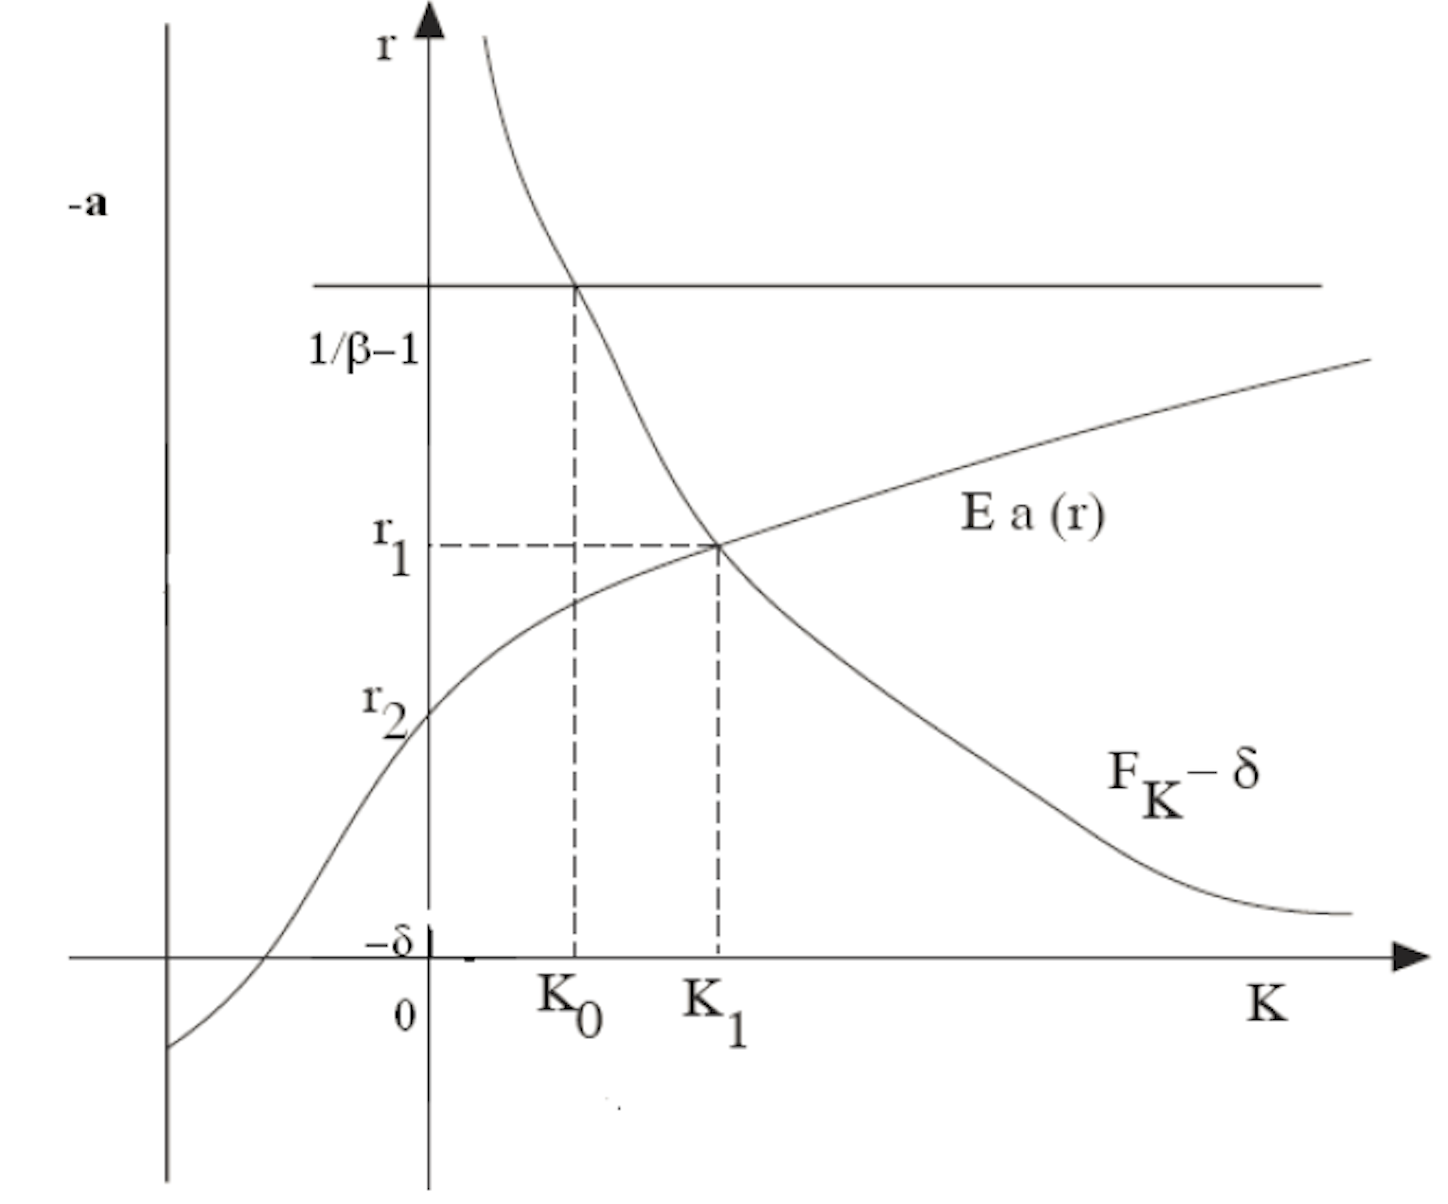
\includegraphics[width=0.65\textwidth]{equilibrium}
\end{center}
\vspace{-0.5em}
\begin{itemize}
\item $K(r)$: firm demand (downward sloping).
\item $A(r)$: household supply (upward sloping, asymptotic to $\rho$ in the complete-markets case).
\item Equilibrium $r^*$ satisfies $K(r^*) = A(r^*)$, with $r^* < \rho$.
\end{itemize}
\end{frame}

\begin{frame}{Probability measures and the Markov operator $Q$}
\begin{itemize}
\item Let $\Lambda$ denote the space of probability measures on the Borel sets of $S = \mathbb{R}_+ \times \mathcal{E}$.
\medskip
\item Define the Markov operator $Q : \Lambda \to \Lambda$ by
\[
(Q\lambda)(B) = \int \mathbb{1}\{(a'(a,\epsilon),\epsilon') \in B\}\,\pi(\epsilon,d\epsilon')\,d\lambda(a,\epsilon).
\]
\medskip
\item Three properties of $Q$ are essential to study the equilibrium:
  \begin{itemize}
  \item \textbf{Feller property} $\to$ existence of an invariant measure.
  \item \textbf{Mixing property} $\to$ uniqueness.
  \item \textbf{Monotonicity} $\to$ convergence.
  \end{itemize}
\medskip
\item These are standard conditions in the Stokey, Lucas \& Prescott (1989, Harvard UP) framework.
\end{itemize}
\end{frame}

\begin{frame}{Feller property $\Rightarrow$ existence}
\textbf{Definition.} $Q$ has the \emph{Feller property} if it maps continuous bounded functions to continuous bounded functions:
\[
f \in C_b(S) \;\Rightarrow\; Q f \in C_b(S).
\]
\medskip
\begin{itemize}
\item Equivalently, the policy $a'(\cdot)$ is continuous in the state.
\medskip
\item Combined with compactness of the state space (or tightness of the orbit), Feller continuity guarantees the \textbf{existence of an invariant measure} via the Krylov--Bogolyubov theorem.
\medskip
\item In Aiyagari, the asset grid is bounded above by $w \epsilon_{\max}/r$ (since saving above this generates negative consumption probability), so $S$ is effectively compact.
\end{itemize}
\end{frame}

\begin{frame}{Mixing property $\Rightarrow$ uniqueness}
\textbf{Mixing condition.} For every two states $s_1, s_2 \in S$, there exist $n_1, n_2 \in \mathbb{N}$ such that the $n$-step distributions $Q^{n_1}\delta_{s_1}$ and $Q^{n_2}\delta_{s_2}$ have overlapping support.
\medskip
\begin{itemize}
\item Intuitively: starting from \emph{any} two initial states, the chain visits a common region in finite time.
\medskip
\item This rules out absorbing sets that would split the state space and admit multiple invariant measures.
\medskip
\item \textbf{Counterexample}: a deterministic policy that pushes any household with $a > a^*$ to $a \uparrow$ and any household with $a < a^*$ to $a \downarrow$ creates two disjoint absorbing sets and \emph{multiple} invariant distributions.
\medskip
\item In standard Aiyagari, idiosyncratic income shocks ensure mixing.
\end{itemize}
\end{frame}

\begin{frame}{Monotonicity $\Rightarrow$ convergence}
\textbf{Monotonicity.} If $\lambda \succeq \lambda'$ in the first-order stochastic dominance sense, then $Q\lambda \succeq Q\lambda'$.
\medskip
\begin{itemize}
\item Combined with Feller and mixing, monotonicity implies that iterating $Q$ from any initial distribution converges to the unique invariant measure $\lambda^*$.
\medskip
\item This is the foundation for \emph{simulating} the model: start from an arbitrary distribution, simulate forward many periods, and read off $\lambda^*$.
\medskip
\item \textbf{Counterexample}: a non-monotone policy can produce stationary distributions that are sensitive to the initial condition; iteration may cycle rather than converge.
\medskip
\item Concavity of the value function and convexity of the budget set yield monotone policies in Aiyagari.
\end{itemize}
\end{frame}

%=============================================================================
\section{Computation of Stationary Equilibrium}

\begin{frame}{Aggregate precautionary savings, applications}
\begin{itemize}
\item Because precautionary saving raises $A(r)$, the equilibrium interest rate satisfies $r^* < \rho = 1/\beta-1$.
\medskip
\item Aggregate capital is \textbf{higher} than in the complete-markets benchmark.
\medskip
\item Standard applications of Aiyagari-style models:
  \begin{itemize}
  \item Wealth and income inequality (top 10\%, Gini, $\ldots$)
  \item Welfare effects of social insurance and tax/transfer policy
  \item Effects of inflation on wealth distribution
  \item Idiosyncratic-risk asset pricing
  \item Quantitative theories of entrepreneurship
  \end{itemize}
\medskip
\item Krueger, Mitman \& Perri (2016, \emph{Handbook of Macro}); Kaplan, Moll \& Violante (2018, \emph{AER}) HANK, $\ldots$
\end{itemize}
\end{frame}

\begin{frame}{Computation of SRCE: three-step algorithm}
\textbf{Goal:} solve for $(r^*, w^*, \lambda^*, v, a', c)$ jointly.
\medskip

\begin{enumerate}
\item \textbf{Step 1.} Fix a candidate $r$. Solve the household dynamic programming problem to obtain $v_r$ and policies $(a'_r, c_r)$.
\medskip
\item \textbf{Step 2.} Given $a'_r$, compute the stationary cross-sectional distribution $\lambda_r$ as the eigenvector of the Markov transition matrix.
\medskip
\item \textbf{Step 3.} Evaluate the excess demand for capital
\[
d(r) \;=\; K(r) - \int a\,d\lambda_r,
\]
and update $r$ via bisection (or Brent) until $|d(r)|<\text{tol}$.
\end{enumerate}
\medskip
This is the \textbf{nested fixed point} that has been the workhorse of HA computation since Aiyagari (1994).\footnote{\scriptsize Classical HA computation methods (endogenous grid method, sparse-grid VFI, transition-matrix methods) are covered in the supplementary video series at \url{https://space.bilibili.com/2142649036/lists/7180709}.}
\end{frame}

\begin{frame}{Step 1: solve the household problem for fixed $r$}
For given $(r,w)$, iterate the Bellman operator
\[
(T_r v)(a,\epsilon) \;=\; \max_{a' \geq -\underline{a}}\!\left\{u\big((1+r)a + w\epsilon - a'\big) + \beta \sum_{\epsilon'} v(a',\epsilon')\,\pi(\epsilon,\epsilon')\right\}
\]
on a grid for $a$.
\medskip
\begin{itemize}
\item Standard tools: VFI with monotonicity exploitation, Howard policy iteration, endogenous-grid method (Carroll), Coleman--Reffett operator.
\medskip
\item Concavity of $u$ and the convex budget set guarantee a unique optimum.
\medskip
\item Output: $a'_r(a,\epsilon)$, $c_r(a,\epsilon)$, $v_r(a,\epsilon)$.
\end{itemize}
\end{frame}

\begin{frame}{Step 2: stationary distribution from the transition matrix}
Discretise $a$ on a grid; combined with $\epsilon$, this gives a finite state space of size $N = N_a \cdot N_\epsilon$.
\medskip

The policy and shock transition induce a Markov matrix $\mathbf{Q}_r \in \mathbb{R}^{N\times N}$ with
\[
\mathbf{Q}_r\big[(a_i,\epsilon_j) \to (a_k,\epsilon_\ell)\big]
= \pi(\epsilon_j,\epsilon_\ell)\cdot\Pr\!\big(a'_r(a_i,\epsilon_j) = a_k\big).
\]
\medskip
The stationary distribution solves
\[
\lambda_r = \mathbf{Q}_r^\top \lambda_r, \qquad \mathbf{1}^\top \lambda_r = 1.
\]
\medskip
Computation: dominant left eigenvector of $\mathbf{Q}_r$, or simply iterate $\lambda \leftarrow \mathbf{Q}_r^\top \lambda$ until convergence (the monotonicity result above guarantees this works).
\end{frame}

\begin{frame}{Step 3: market clearing on $r$}
With $\lambda_r$ in hand, compute the household supply of capital
\[
A(r) \;=\; \sum_{i,j} a_i \,\lambda_r(a_i,\epsilon_j),
\]
and compare to firm demand:
\[
d(r) \;=\; K(r) - A(r).
\]
\medskip
\textbf{Update rule}:
\begin{itemize}
\item If $d(r) > 0$: capital is scarce, raise $r$.
\item If $d(r) < 0$: capital is abundant, lower $r$.
\item Bisection or Brent's method converges in $O(\log(1/\text{tol}))$ outer iterations.
\end{itemize}
\medskip
Each outer iteration requires solving Steps 1 and 2 from scratch --- the dominant cost.
\end{frame}

\begin{frame}{Implementation details}
\begin{itemize}
\item \textbf{Asset grid}: dense near the borrowing constraint where the policy bends; sparse for high $a$. Often log-spaced.
\medskip
\item \textbf{Initial value function}: zero, or the closed-form complete-markets value, or the value from the previous outer iteration.
\medskip
\item \textbf{Multigrid}: solve on a coarse grid first, then interpolate onto a finer grid as a warm start.
\medskip
\item \textbf{Acceleration}: Howard's policy iteration steps, modified policy iteration, endogenous grid method (Carroll, 2006, \emph{Economics Letters}).
\medskip
\item \textbf{Convergence criterion}: $\|v^{(n+1)} - v^{(n)}\|_\infty < \varepsilon_v$ inside; $|d(r)| < \varepsilon_r$ outside.
\end{itemize}
\end{frame}

\begin{frame}{Numerical challenges and the curse of dimensionality}
\begin{itemize}
\item For Aiyagari, the per-iteration state space is $\mathbb{R}_+ \times \mathcal{E}$ --- 2 continuous dimensions, manageable on a grid.
\medskip
\item Real-world quantitative HA models often have:
  \begin{itemize}
  \item Multiple assets (liquid + illiquid in HANK; portfolio choice).
  \item Multidimensional idiosyncratic states (income, unemployment, family structure).
  \item \emph{Aggregate} shocks $\to$ the cross-sectional distribution becomes part of the state (Krusell--Smith).
  \end{itemize}
\medskip
\item With $d$ continuous individual states and $N_a$ grid points per dimension, total points are $N_a^d$ --- the \textbf{curse of dimensionality}.
\medskip
\item This is where machine learning, and in particular deep neural networks, become indispensable.
\end{itemize}
\medskip
\emph{Next (T2a):} neural-network function approximation and the Euler-residual loss on a toy optimal-growth model.
\end{frame}

\end{document}
